 % LuaLaTeX文書; 文字コーAドはUTF-8
 \documentclass[unicode,12pt, A4j]{ltjsarticle}% 'unicode'が必要
 %\usepackage{luatexja}% 日本語したい
 \usepackage{luatexja-fontspec}
 %\usepackage[hiragino-pron]{luatexja-preset}% IPAexフォントしたい(ipaex)
 \usepackage[hiragino-pron,deluxe,expert,bold]{luatexja-preset}
\usepackage{tikz}
\usetikzlibrary{arrows.meta}
\usetikzlibrary{calc}
\usepackage{ifthen}
 \usepackage[english]{babel}%多言語文書を作成する
 \usepackage{amsmath,amssymb}%標準数式表現を拡大する
 \usepackage{physics}
 \usepackage[subpreambles=true,sort=true]{standalone}
% \renewcommand{\kanjifamilydefault}{\gtdefault}% 既定をゴシック体に
 \usepackage[backend=bibtex,style=phys,articletitle=false,biblabel=brackets,chaptertitle=false,pageranges=false]{biblatex}
 %\usepackage[style=authoryear,backend=bibtex]{biblatex}


 \usepackage{mhchem}
 % あとは欧文の場合と同じ




  \usepackage{caption}
  \usepackage[subrefformat=parens]{subcaption}
\title{東大数学理科後期1997年度}
\author{}
\date{}

\begin{document}
\maketitle

\section{問題1}
右の図のように、1辺の長さが1の正三角形で、平面を分割する。これらの1辺の長さが1の正三角形1つ1つを、単位正三角形とよぶことにする。は
じめに1個以上有限個の単位正三角形が塗りつぶされているとし、以下の操作を繰り返すことにより、次々に単位正三角形を塗りつぶしていく。

『1回の操作ごとに、既に塗りつぶされている単位正三角形と少なくとも1つの辺を共有する単位正三角形を、すべて塗りつぶす』

次の問いに答えよ。

\begin{enumerate}
 \item はじめに塗りつぶされている単位正三角形が1つだけのとき、$n$回目の操作が終わったときに塗りつぶされている単位正三角形の個数 $a_n$ を求めよ。
 \item はじめに2個以上有限個の単位正三角形が塗りつぶされているとき、$n$回目の操作が終わったときに塗りつぶされている単位正三角形の個数を $b_n$ とおくと、極限
\begin{align}
\lim_{n \to \infty} \frac{a_n}{b_n}
\end{align}
は、はじめの塗りつぶされ方がどのようであっても存在するか。極限が存在する場合については、その極限値を求めよ。存在しない場合があるならば、その例をあげよ。
\end{enumerate}

\begin{figure}[h]
\centering 
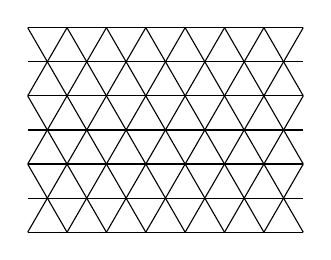
\begin{tikzpicture}[scale=0.5]
% Drawing triangular grid
% Drawing triangular grid with equilateral triangles
\clip (-0.5,0) rectangle (6.5,0.866*6);

\foreach \i in {0,...,6} {
        % Horizontal lines
        \draw (-0.5, {0.866*\i}) -- (6.5, {0.866*\i});
}
\foreach \k in {-4,...,10} {
% 斜め線
    \draw ({-0.5+\k}, 0) -- ({-0.5+\k - 0.5*6}, {0.866*6});  % 傾き60度(右上がり)
    \draw ({-0.5+\k}, 0) -- ({-0.5+\k + 0.5*6}, {0.866*6}); % 傾き120度(左上がり)
}
\end{tikzpicture}
\end{figure}



\section{問題2}
座標平面上の点 $A(x,y)$ が次の連立不等式の表す領域を動くとする。

\begin{align}
 \begin{cases}
|xy| < 1 \\
y > 0
\end{cases}
\end{align}

関数 $y = \frac{1}{|x|}$ のグラフのうち、$x < 0$ の部分を $H$, $x > 0$ の部分を $K$ とする。点 $A$ に対し、$x$ 軸上の2点 $B$, $C$, 曲線 $H$ 上の点 $D$, 曲線 $K$ 上の点 $E$ を次の条件によって定める。

『直線 $AB$ は、2点 $A$, $B$ の間の点 $D$ で曲線 $H$ に接し、直線 $AC$ は、2点 $A$, $C$ の間
の点 $E$ で曲線 $K$ に接する』

\begin{enumerate}
 \item 三角形 $ABC$ の面積のとり得る範囲を求めよ。
 \item 三角形 $ADE$ の面積のとり得る範囲を求めよ。
\end{enumerate}

\section{問題3}
ボタンを1回押す毎に、1以上$N$以下の整数を、同じ確率で1つずつ発生する機械がある。複数回ボタンを押した場合、どの整数が発生するかについての確率は、どの回についても他の回とお互いに独立であるとする。この機械には、発生した整数の下4桁のみを表示する表示装置が接続されており、4桁未満の数については、欠けている桁に0を入れて4桁にして表示される。たとえば、発生した整数が925のときは0925が、12320のときは2320が表示される。

2回ボタンを押したとき、同じ数字が表示される確率を $p_N$ とする。

(1) \quad $p_{10000}$ を求めよ。

(2) \quad $p_{10000}$ と $p_{10001}$ は、どちらが大きいかを判断し、その差を有効数字4桁で求めよ。

(3) \quad 確率 $p_{10000}, p_{10001}, \cdots, p_{20000}$ のうち、最小の値を $q$, 最大の値を $r$ とおく。 $q$ と
$r$ を求めよ。

(4) \quad $N$ を 10000 以上の整数とするとき、$q \leq p_N \leq r$ を示せ。

\end{document}